\documentclass[12pt,a4paper]{article}
\usepackage[T1]{fontenc}
\usepackage{amsmath}
\usepackage{amssymb}
\usepackage{graphicx}
\usepackage[UTF8,heading=true]{ctex}
\usepackage{geometry}
\usepackage{diagbox}
\usepackage[]{float}
\usepackage{xeCJK}
\usepackage{indentfirst}
\usepackage{multirow}
\usepackage[section]{placeins}
\usepackage{caption}
\usepackage{cite}
\usepackage{graphics}
\usepackage{subfig}

\graphicspath{{./figure/}}

\setCJKfamilyfont{zhsong}[AutoFakeBold = {5.6}]{STSong}
\newcommand*{\song}{\CJKfamily{zhsong}}

\geometry{a4paper,left=2cm,right=2cm,top=0.75cm,bottom=2.54cm}

\newcommand{\experiName}{虚拟仪器}%实验名称
\newcommand{\supervisor}{}%指导教师
\newcommand{\name}{张钰堃}
\newcommand{\studentNum}{2022K8009926020}
\newcommand{\class}{2}%班级
\newcommand{\group}{08}%组
\newcommand{\seat}{11}%座位号
\newcommand{\dateYear}{2023}
\newcommand{\dateMonth}{10}%月
\newcommand{\dateDay}{31}%日
\newcommand{\room}{教学楼702}%地点
\newcommand{\others}{$\square$}

\ctexset{
    section={
        format+=\raggedright\song\large
    },
    subsection={
        name={\quad,.}
    },
    subsubsection={
        name={\qquad,.}
    }
}

\begin{document}
\noindent

\begin{center}

    \textbf{\song \zihao{-2} \ziju{0.5}《基础物理实验》实验报告}
    
\end{center}


\begin{center}
    \kaishu \zihao{5}
    \noindent \emph{实验名称}\underline{\makebox[28em][c]{\experiName}}
    \emph{指导教师}\underline{\makebox[9em][c]{\supervisor}}\\
    \emph{姓名}\underline{\makebox[6em][c]{\name}} 
    \emph{学号}\underline{\makebox[14em][c]{\studentNum}}
    \emph{分班分组及座号} \underline{\makebox[5em][c]{\class \ -\ \group \ -\ \seat }\emph{号}} (\emph{例}:\,1- 04- 5\emph{号})\\
    \emph{实验日期} \underline{\makebox[3em][c]{\dateYear}} \emph{年}
    \underline{\makebox[2em][c]{\dateMonth}}\emph{月}
    \underline{\makebox[2em][c]{\dateDay}}\emph{日}
    \emph{实验地点}\underline{{\makebox[4em][c]\room}}
    \emph{调课/补课} \underline{\makebox[3em][c]{否}}
    \emph{成绩评定} \underline{\hspace{8em}}
    {\noindent}
    \rule[5pt]{17.7cm}{0.2em}

\end{center}

\section{实验目的}
    1.了解虚拟仪器的概念;\par
    2.了解图形化编程语言LabVIEW,学习简单的LabVIEW编程;\par 
    3.完成伏安法测电阻的虚拟仪器设计\par

\section{实验仪器}
计算机(含操作系统),LabVIEW 2014,NI ELVIS Ⅱ+,导线若干,元件盒一个($100 \Omega $标准电阻一个,待测电阻2个,稳压二极管一个)
\section{实验原理}
    \subsection{综述}
使用计算机对专用硬件(集合多种仪器且为开源)进行编程,以计算机为中心进行测量。由于实验平台为开源,编程的多样化,使实验仪器相对传统仪器更加灵活,功能更加多样。\par
    \subsection{硬件}
本实验使用的硬件平台是个人电脑(PC机),美国国家仪器公司(National Instruments)的教学实验室虚拟仪器套件(Educational Laboratory Virtual Instrumentation Suite)II+(缩写为NI ELVISⅡ+)和自带的原型板。\par
虚拟仪器综合实验平台ELVIS Ⅱ+,集成8路差分输入(或16路单端输入)模拟数据采集通道、24路数字I/O通道,以及多款常用的仪器(包括示波器、数字万用表、函数发生器、动态信号分析仪、
二线电流电压分析仪、三线电流电压分析仪、阻抗分析仪、VPS电源等)。平台通过USB连接PC。虚拟仪器综合实验平台是开源的,可以在LabVIEW 中进行定制,
同时可以使用LabVIEW Express VI 和LabVIEW Signal Express 的步骤对设备进行编程。\par
    \subsection{软件}
本实验使用的用于虚拟仪器系统设计的软件开发平台是LabVIEW (laboratory virtual instrument engineering workbench)。它将计算机数据分析和显示能力与仪器驱动程序整合在一起,为针对仪器的编程提供了很大的便利。
而且, LabVIEW是一种图形化编程语言,编程过程也就是设计流程图,即使初学者也能很快入门。\par
用LabVIEW开发平台编制的虚拟仪器程序简称为VI。 VI包括三个部分:前面板(front panel)、程序框图(Block diagram)和图标/连线板。\par
前面板用于设置输入数值和显示输出量,相当于真实仪表的前面板。前面板上的图标,分为两类:输入类(Controls,用于输入)和显示类(Indicators,用于输出),具体可以是开关、旋钮、按钮、图形、图表等表现形式。
程序框图相当于仪器的内部功能结构,其中的端口用来和前面板的输入对象和显示对象传递数据,节点用来实现函数和功能子程序调用,图框用来实现结构化程序控制命令,连线则代表程序执行过程中的数据流。\par
    \subsection{利用虚拟仪器测量伏安特性}
本实验中利用一个模拟输出通道为整个测量电路供电,利用两个模拟输入通道分别测量总电压和标准电阻上的电压;
利用测量得到的电压数值和标准电阻数值就可以得到电路中的电流以及待测电阻上的电压。在程序控制下,电路电压由0 V开始逐渐增加到设定电压,电压每改变一次,测得一组电压电流值,最后得到一个数组,经过线性拟合后就可以得到待测电阻值。使用单端输入方式时,
各个输入通道共用地线,各通道测量的都是对地的电压,连线时要加以注意。也可使用差分输入。

\section{实验内容}
    \subsection{初步熟悉LabVIEW开发环境的基本操作和编程方法}
    选择文件→新建 VI进入LabVIEW环境。我们会看到前面板和程序框图。利用ctrl+T快捷键可以将二者并置。
    选择控件选板上这些图标并放置在前面板上,相应的端子和图标会出现在程序框图上。通过这些控件图标可以通过前面板控制程序中的数据,或者将程序运行结果显示出来。在程序框图窗口中,
    利用函数选板提供的循环、数学运算、比较以及公式节点等函数功能可以创建框图程序。

    \subsection{创建一个模拟温度测量程序}
    假设传感器的输出电压和温度成正比。那么可以利用程序根据电压计算温度。同时我们希望程序中可以用开关切换摄氏温度值和华氏温度值的显示。
    我们使用一个输入控件来代替数据采集卡对传感器的测量结果。再将电压读数乘以100转换成华氏温度读数,或者再把华氏温度转换成摄氏温度。

    \subsubsection{创建前面板}
    新建一个空白VI,打开前面板窗口,在空白处点右键,弹出控件选板,在控件选板中选择下列控件,放在前面板上,添加各控件的名称以及开关状态的标识。\par
    放入温度计(控件→数值→温度计)。\par
    放入垂直滑动杆开关(控件→布尔→垂直滑动杆开关);用标签工具将名称改为“温度值单位”。在垂直滑动杆开关上点击右键,
    在快捷菜单中选择显示项→布尔文本,让开关的状态显示出来。使用标签工具,在开关的“条件真”位置旁边输入自由标签“摄氏”,再在“条件假”位置旁边输入自由标签“华氏”。\par
    放入数值显示控件(控件→数值→数值显示控件)用标签工具将名称改为“温度值”\par
    放入数值输入控件(控件→数值→数值输入控件)用标签工具将名称改为“采集的电压”。这里只是简单地用一个输入控件代替采集的电压值。\par

    \subsubsection{创建程序框图}
    打开程序框图。在函数选板中找到下列对象并将其放入程序框图中:\par
    放入乘法函数、减法函数、除法函数(函数→数值)。\par
    放入选择函数(函数→比较)。根据温标选择开关的值输出华氏温度(当选择开关为假)或者摄氏温度(选择开关为真)数值。该函数有两个数值型输入端t和f,一个布尔型输入端s;当s为真时,输出值为t;当s为假时,输出值为f。\par
    将所需要的对象放入程序框图中之后,把图标移至如图7所示的位置,再用连线工具连接起来,并在需要的地方创建数值常量(用连线工具,
    右键单击你希望连一个常量的对象连线端子,在快捷菜单中选择创建→常量,即可创建一个与端口数据类型相匹配的常数。也可以先放入一个数值常量再连线。\par
    整个程序创建完毕。最后可以整理一下图标位置和连线(在需要整理的连线上单击右键,在快捷菜单中选择整理连线)。\par
    
    \begin{figure}[H]
        \centering
        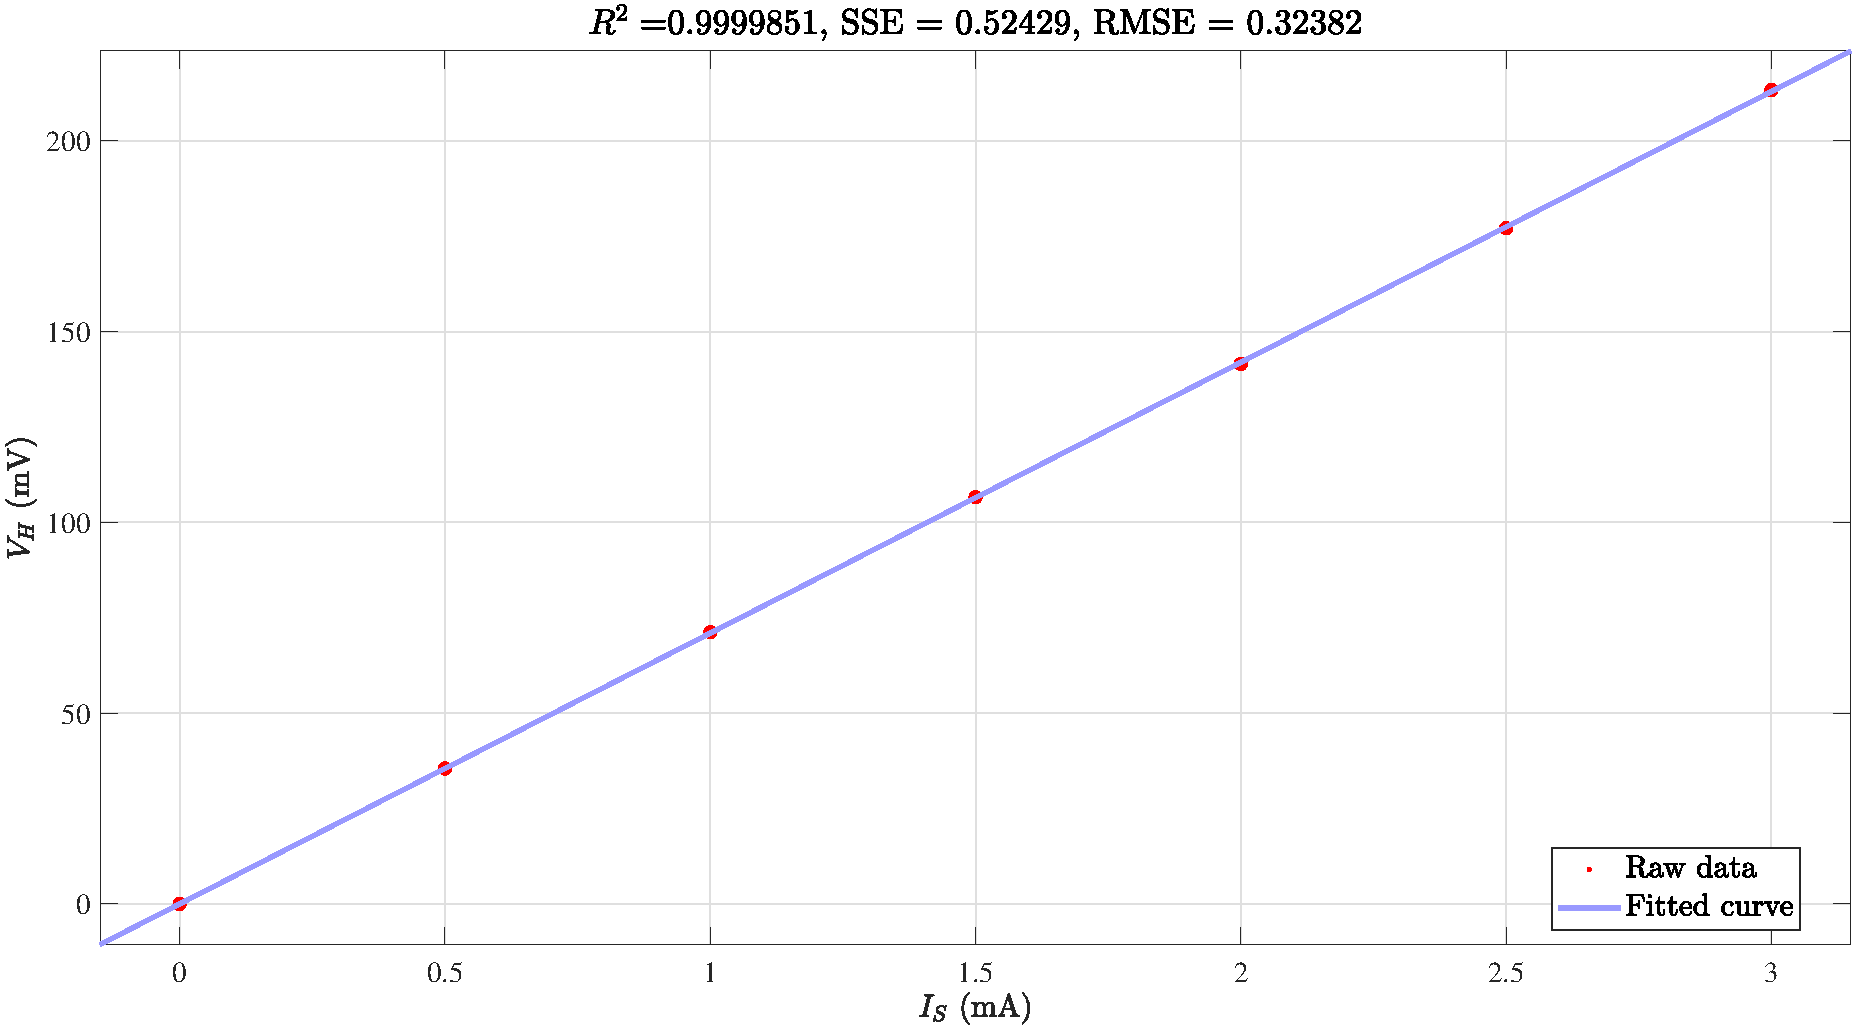
\includegraphics[scale=0.3]{1.jpg}
    \end{figure}
    \subsubsection{运行程序}
    选择前面板窗口,运行VI程序。点击连续运行按钮,使程序运行于连续运行模式。
    改变“采集的电压”控件输入值
    和温度值单位,观察程序运行情况。
    再点击连续运行按钮,停止程序运行。用文件菜单的保存功能(或<Ctrl+S>快捷键)保存上述文件。

    \subsection{制作改进版温度计}
    \subsubsection{创建前面板}
    前面板在前一个实验的基础上放上一个Express XY 图(控件选板→图形→Express XY 图)。去掉
    “采集的电压”,在相同的位置放上一个数值显示控件,用标签工具将名称改为“测量的电压”。再加上
    一个停止运行的按钮

    \subsubsection{创建程序框图}
    根据讲义内容先将减法、乘法、除法和数值放入程序框图中。然后加入等待控件。\par
    在程序框图放入一个“创建数组”,拖放其图标使其有两个输入端。\par
    加入随机数,作为被测量的电压。然后根据讲义中的图片将线连好
    \begin{figure}[H]
        \centering
        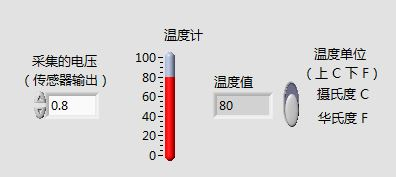
\includegraphics[scale=0.3]{3.jpg}
    \end{figure}
    \subsubsection{运行程序}
    选择前面板窗口,运行VI程序。点击连续运行按钮,使程序运行于连续运行模式。改变
    温度值单位,观察程序运行情况。再点击连续运行按钮,停止程序运行。用文件菜单的保存功能(或<Ctrl+S>快捷键)保存上述文件。

    \subsection{创建一个电压输出和采集的程序}
    \subsubsection{编写输出电压程序}
    新建一个空白的VI,在程序框图中创建虚拟通道。在程序框图中打开函数选板,选择测量I/O→DAQmx - 数据采集→DAQmx创建虚拟通道。
    把该图标放在程序框图中,右键点击,在弹出菜单中选择选择类型→模拟输出→电压。将鼠标设为连线工具或自动选择工具,并放在该图标左上边框位置,
    当弹出“物理通道”时,右键点击,在弹出菜单中选择创建→输入控件。在函数→测量I/O→DAQmx-数据采集中,分别选择“DAQmx开始任务”、“DAQmx写入”和“DAQmx清除任务”节点放入程序框图中。
    在“DAQmx写入”的图标数据输入端创建输入控件。

    创建一个While循环,在函数选板中,选择“结构”→“While循环”。在程序框图中选择函数选板中的“定时→等待100 ms”,并创建常量。
    在前面板中创建停止按钮,并将“等待100 ms”和停止按钮放在While循环内。记得用连线工具将相应的端口连接起来。

    \subsubsection{编写采集电压程序}
    用类似的方法创建电压采集程序。整理各图标和连线。
    \begin{figure}[H]
        \centering
        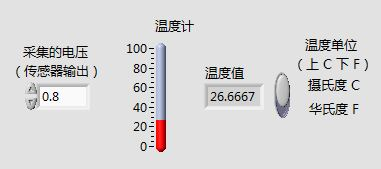
\includegraphics[scale=0.3]{2.jpg}
    \end{figure}
    \subsubsection{运行程序}
    打开ELVIS电源和原型板电源。在前面板上设置输出通道为Dev6/ao0,输入通道为Dev6/ai0。
    在原型板上用导线连接模拟输出(Analog Outputs)“AO 0”端和模拟输入(Analog Input Signals)“AI 0 +”端,将“AI 0 -”端和接地端“AIGND” 用导线连接。

    在前面板窗口,运行VI程序。改变输出电压,观察测量电压的变化。可点击停止按钮,观察程序运行情况。

    结束后,停止程序运行。保存上述文件。

    \subsection{用虚拟仪器测量伏安特性}
    \subsubsection{创建前面板}
    放上一个Express XY 图(控件选板→图形→Express XY 图),用于显示电压—电流图。
    将名字改成“电阻的伏安曲线图”,并将纵坐标和横坐标分别改成“电流(A)”和“电压(V)”。
    在图的右上角曲线0处点右键,选择常用曲线,选“点+线”模式。

    放入四个数值型输入控件,分别将名称改为“输出电压步长”、“测量数据点数”、“标准电阻”、“时间间隔”。
    在“时间间隔”上点右键,选择显示项→单位标签,此时会在控件右方出现一个光标,直接输入“s”,这样时间间隔成为一个单位为s的量。
    时间间隔用来设置电压改变和测量数据之间的时间间隔,让电路达到平衡再进行测量。

    放入一个数值型显示控件(用于显示电阻测量值),并将名称改为“待测电阻值”

    加入一个二维数组显示控件,用于显示测量的电压和电流。先放入数组控件(控件选板→“数组、矩阵与簇”→“数组”),
    再将它变成数值型的数组显示控件(创建一个数值型显示控件把它拖放到数组框内),
    再改变数组维数为二维(用定位工具向下拖拽索引框使它有两个索引值,或者在索引框上点击右键呼出快捷菜单选择“添加维度”。
    把数组的名字改成“数据”。放入一个开关按钮(控件→布尔→开关按钮),用于控制程序进程。

    \subsubsection{创建程序框图}
    根据实验思路,先输出一个电压,等到稳定后测量。控制程序执行顺序可以通过顺序结构来实现。
    在程序框图中放入一个平铺式顺序结构。在其边框上点击鼠标右键,选择弹出菜单中的“在后面添加帧”使顺序结构有5帧。
    之前在程序框图中已经有一些控件图标,它们对应于前面板上的各个控件,现在可以把这些图标移动到顺序结构各帧之中。

    首先,让ELVIS输出电压。在第0帧中放入一个“DAQ助手”(函数→Express→输出→DAQ助手)用于输出电压。
    在弹出窗口中选择:生成信号→模拟输出→电压,然后在自动弹出的物理通道选择窗口中选Dev3(NI ELVIS II+)下的“ao 0”,
    点击完成。在弹出的DAQ助手窗口中的左下角“生成模式”项目下选“1采样(按要求)”,在该窗口的右下角点击确定。

    让程序等待一段时间。在第1帧中放入一个“等待(ms)”用于等待电阻上的电流达到稳定;再放入一个“单位转换”(在函数→数值→转换下),
    在模块中键入“ms”,用于将单位s转换成ms,将“单位转换”的输入端和“时间间隔”相连,输出端和“等待(ms)”端相联。

    用ELVIS采集总电压和标准电阻上的电压,计算待测电阻上的电压、电流值。

    在第2帧中放入一个“DAQ助手”,在弹出窗口中选择采集信号→模拟输入→电压,
    在自动弹出的物理通道选择窗口中选Dev3(NI ELVIS II+)下的“ai 0”和“ai 1”,点击完成。
    在弹出的DAQ助手窗口中的左下角“生成模式”项目下选“1采样(按要求)”

    接下来在第2帧中放入两个索引数组(函数→数组→索引数组)。用连线工具将DAQ中的数据输出端和数组中的数据端相连,
    在“索引数组”左下角的索引端创建常量,分别将上下两个索引常量设为0和1。再在第2帧中放入“减”和“除”的节点。
    用总电压减去标准电阻上的电压得出待测电阻上的电压,再把标准电阻上的电压除以标准电阻,求出电流。

    再让程序等待一段时间,以减少对数据测量过程的影响。在第3帧中放入“等待(ms)”,在输入端点右键创建常量,将常量数值改为100(表示100 ms)。

    在第4帧中放入一个“DAQ助手”,使顺序结构结束时电压输出为0。

    通过While循环来实现电压的改变:放入的While循环要包含先前的顺序结构、“数据”和“电阻的伏安曲线图”。在“函数”→“结构”→“While循环”下单击选择While 循环,
    然后在程序框图中,在顺序结构左上角以外点击鼠标左键,向顺序结构右下角拖拉while循环框,将顺序结构等对象完全包含之后再点鼠标左键,
    这样就把顺序结构等放在了While循环中。或者,先放一个空的While循环。再用定位工具拉出一个框框住整个顺序结构,把它拖进While循环中。
    我们希望ELVIS输出电压从0 V开始到 5 V,每隔0.25 V测一次。对于较小的待测电阻,这些值要用更小的值,以保证电流不超过限制。
    可以把While循环框左下角的循环变量i和数值型控件“输出电压步长”相乘,将其乘积和顺序结构第0帧中的DAQ助手的数据端相连。

    While循环的循环变量i从0开始计数;循环条件在框内语句都执行之后才进行判断,因此While循环至少执行一次。
    可以把While循环的i和输入型控件“测量数据点数”中的值作比较,在和开关作逻辑“与”运算后和While框内右下角的循环条件端子相连,
    用于控制循环。注意把循环条件改为“真时继续”。

    用移位寄存器实现数据的实时显示,移位寄存器的功能是在相邻两次循环之间传递数据。
    在While循环左边框(或右边框)上点右键选择“添加移位寄存器”加上两个移位寄存器,
    分别用来存储并传递电压和电流的测量数据。在循环中放入两个“创建数组”(函数→数组→创建数组)。
    向下拖放其图标使其有两个输入端,将上方的“元素”端口和左边的移位寄存器相连、下方“元素”端口和电压(或是电流)相连,
    输出端“添加的数组”和右端的移位寄存器相连。此处创建数组的作用是将来自元素输入端的新测量数据与数组输入端的原来一维数组中的数据串成一个新的一维数组。
    注意在左右两端移位寄存器之间的线完全连好以前,连线会显示为断线;两边都连好之后,
    连线才会显示正常。分别在左边两个移位寄存器的小三角上点右键,选择创建→常量,
    创建两个空的数组,用于初始化数据。

    显示测量数据。在程序框图放入一个“创建数组”,拖放其图标使其有两个输入端,把连到移位寄存器上的电压和电流分别和“创建数组”的输入端相连,
    把“创建数组”的输出和名为“数据”的数组显示控件相连

    显示伏安曲线。把电压数组和“创建 XY图”的X输入相连,电流数组和Y 输入相连。由于显示数
    组控件“数据”和显示图形控件“电阻的伏安曲线图”都在While循环以内,因此每次循环“数据”和“电阻的伏安曲线图”都会更新一次。

    计算电阻值。在循环外面放入一个“线性拟合”节点(函数→数学→拟合→线性拟合),将移位寄存器传
    递出来的电流数组和“线性拟合”的X输入端相连,电压数组和Y输 入端相连,把“线性拟合”的“斜
    率”输出端和“待测电阻值”显示控件相连,显示电阻值。

    在前面板上整理各图标位置;在程序框图中检查并整理连线。保存程序。

    \subsubsection{正确连接外部电路}
    在ELVIS自带的原型板上连接电路。电压的模拟输出和模拟采集在原型板的左侧。
    \begin{figure}[H]
        \centering
        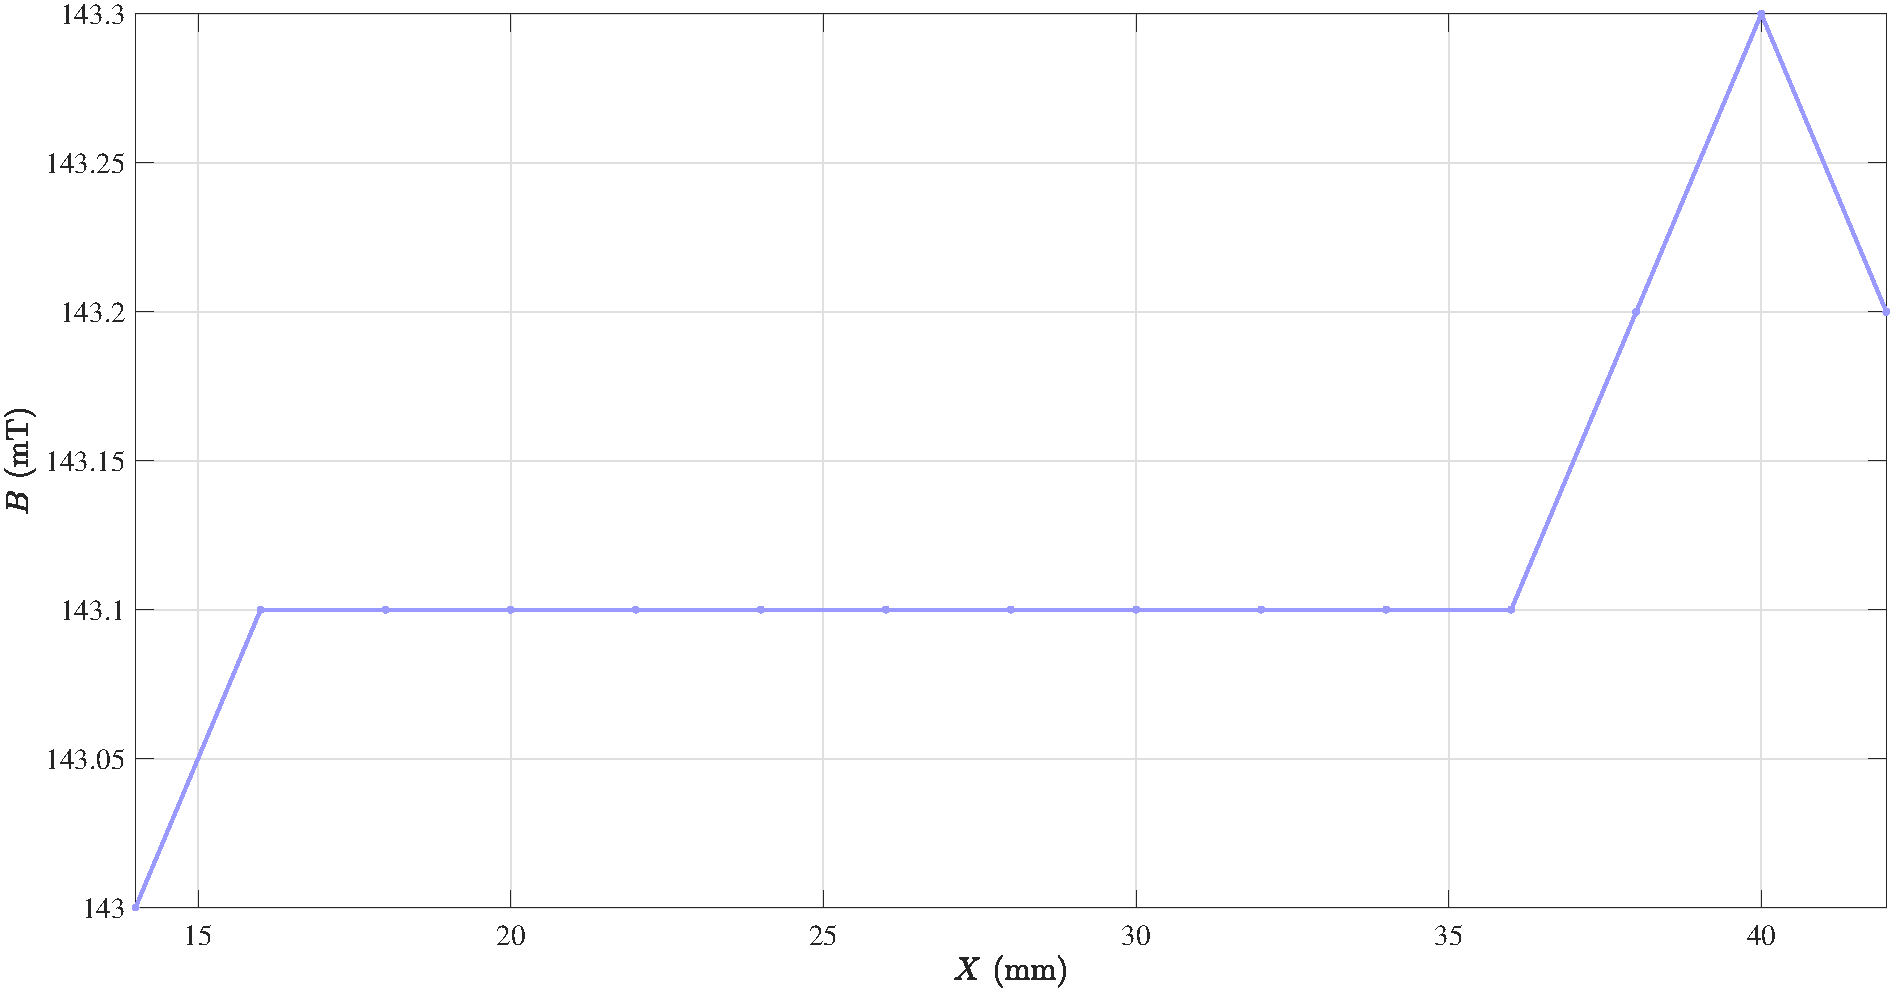
\includegraphics[scale=0.3]{4.jpg}
    \end{figure}
    \subsubsection{运行程序}
    再次检查前面板窗口中各参量设置情况,运行程序。分别测量两个待测电阻的电阻值。分析实验结果。

    \subsubsection{利用前面的程序测量并绘制稳压二极管伏安特性曲线}
    改变“输出电压步长”为负值时,可以在电阻两端加反向电压。

\section{实验数据及处理}
\begin{figure}[H]
    \centering
    \caption{实验4电路}
    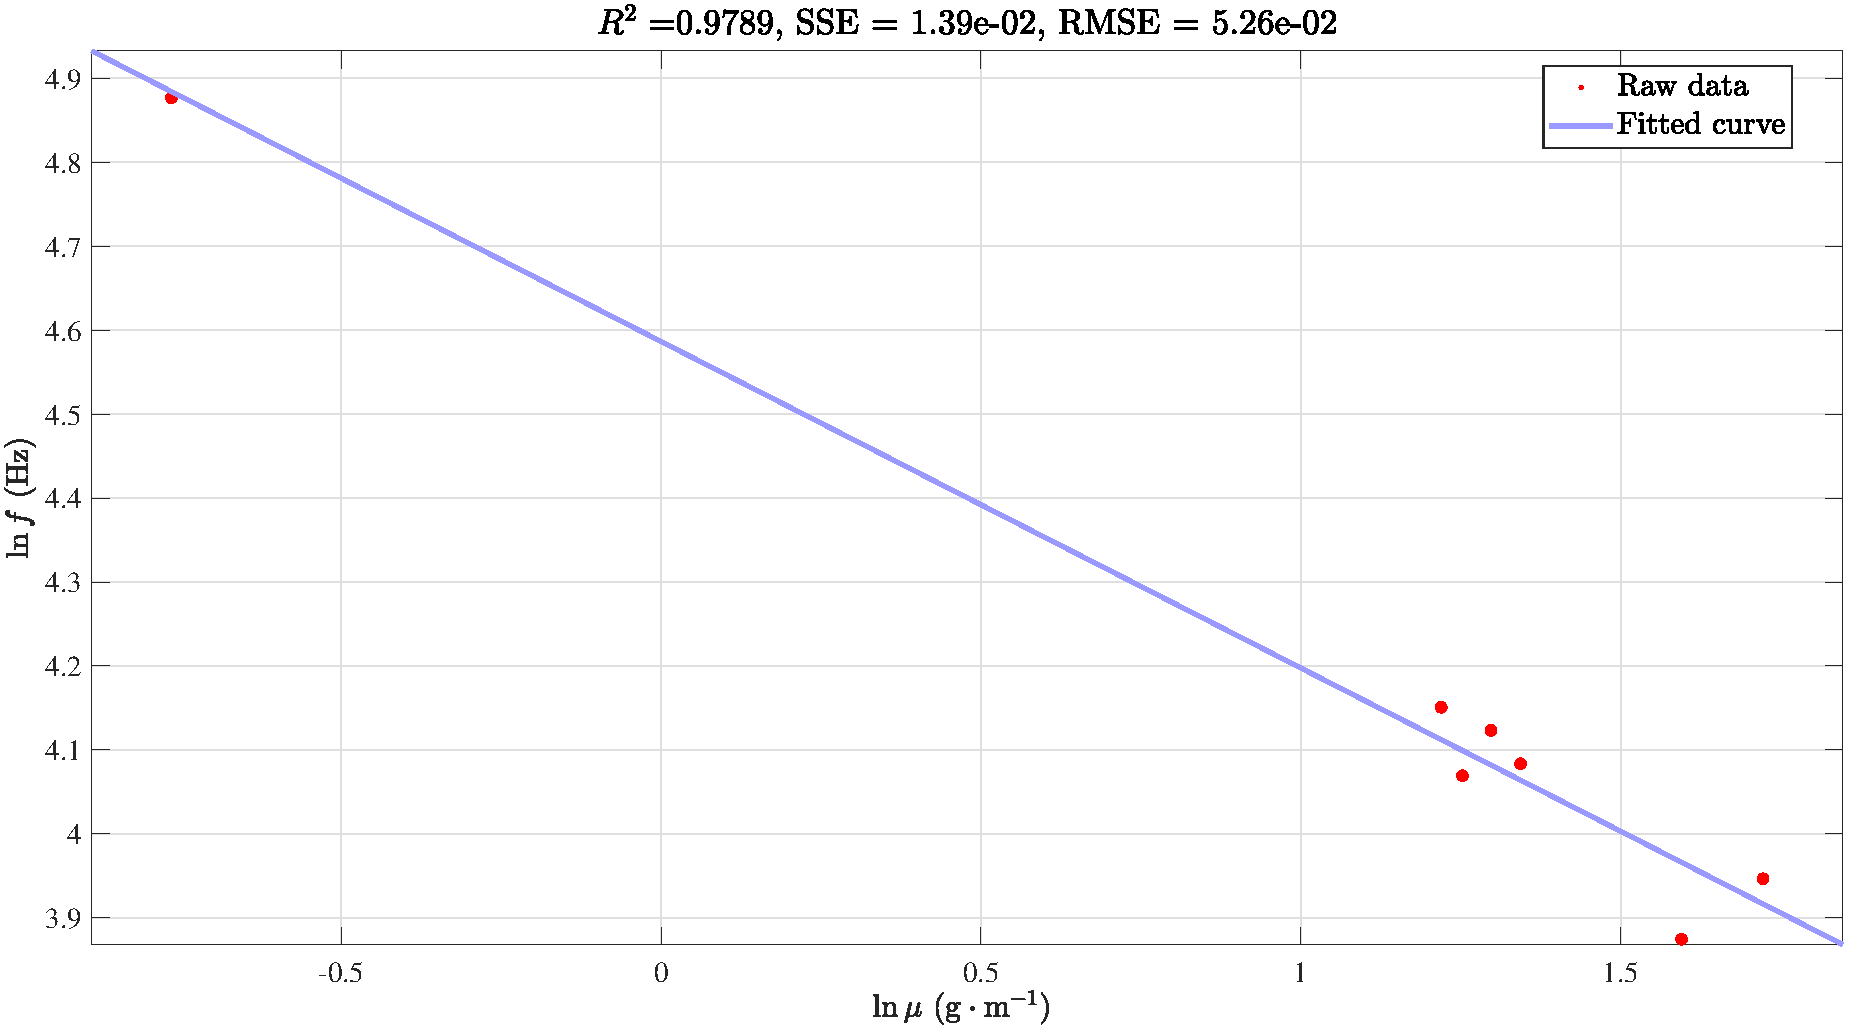
\includegraphics[scale=0.3]{5.jpg}
\end{figure}
    为了表示方便,以下数据均保留三位有效数字并对单位做了处理。

\begin{figure}[H]
        \centering
        \caption{数据表格}
        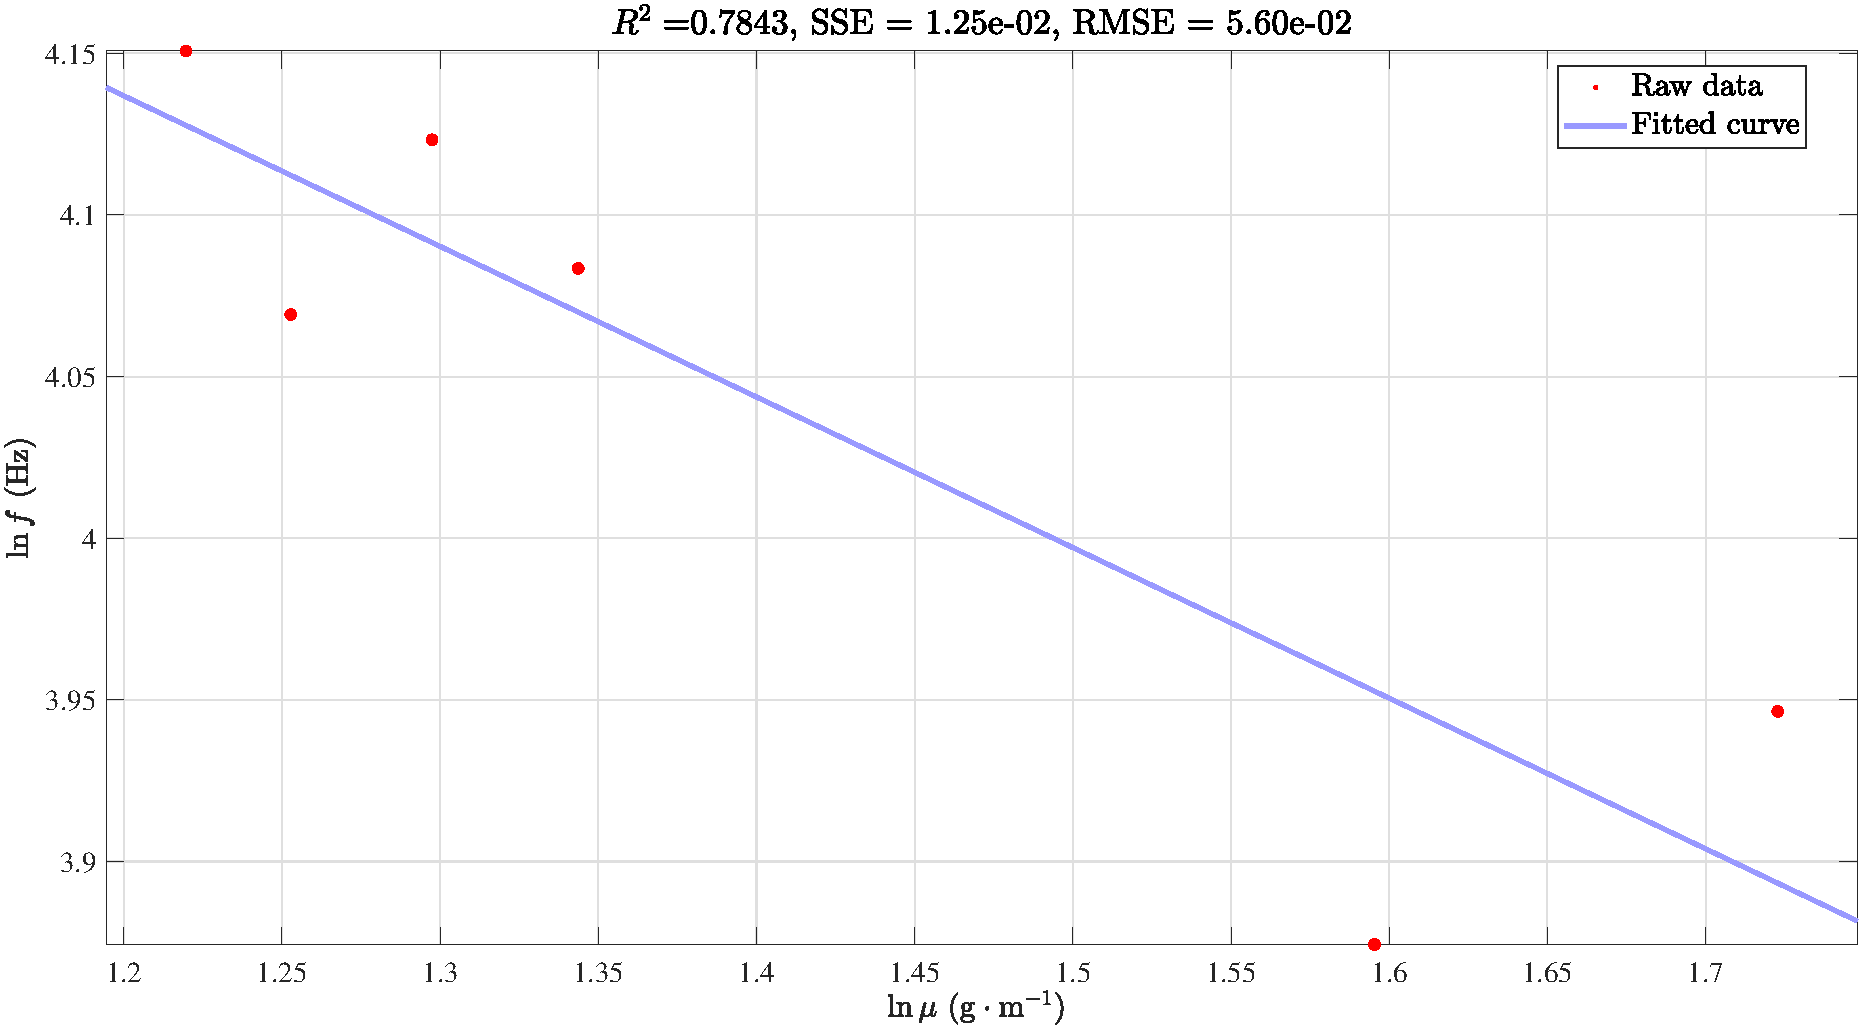
\includegraphics[scale=0.7]{6.png}
\end{figure}

\begin{figure}[H]
    \centering
    \caption{数据曲线}
    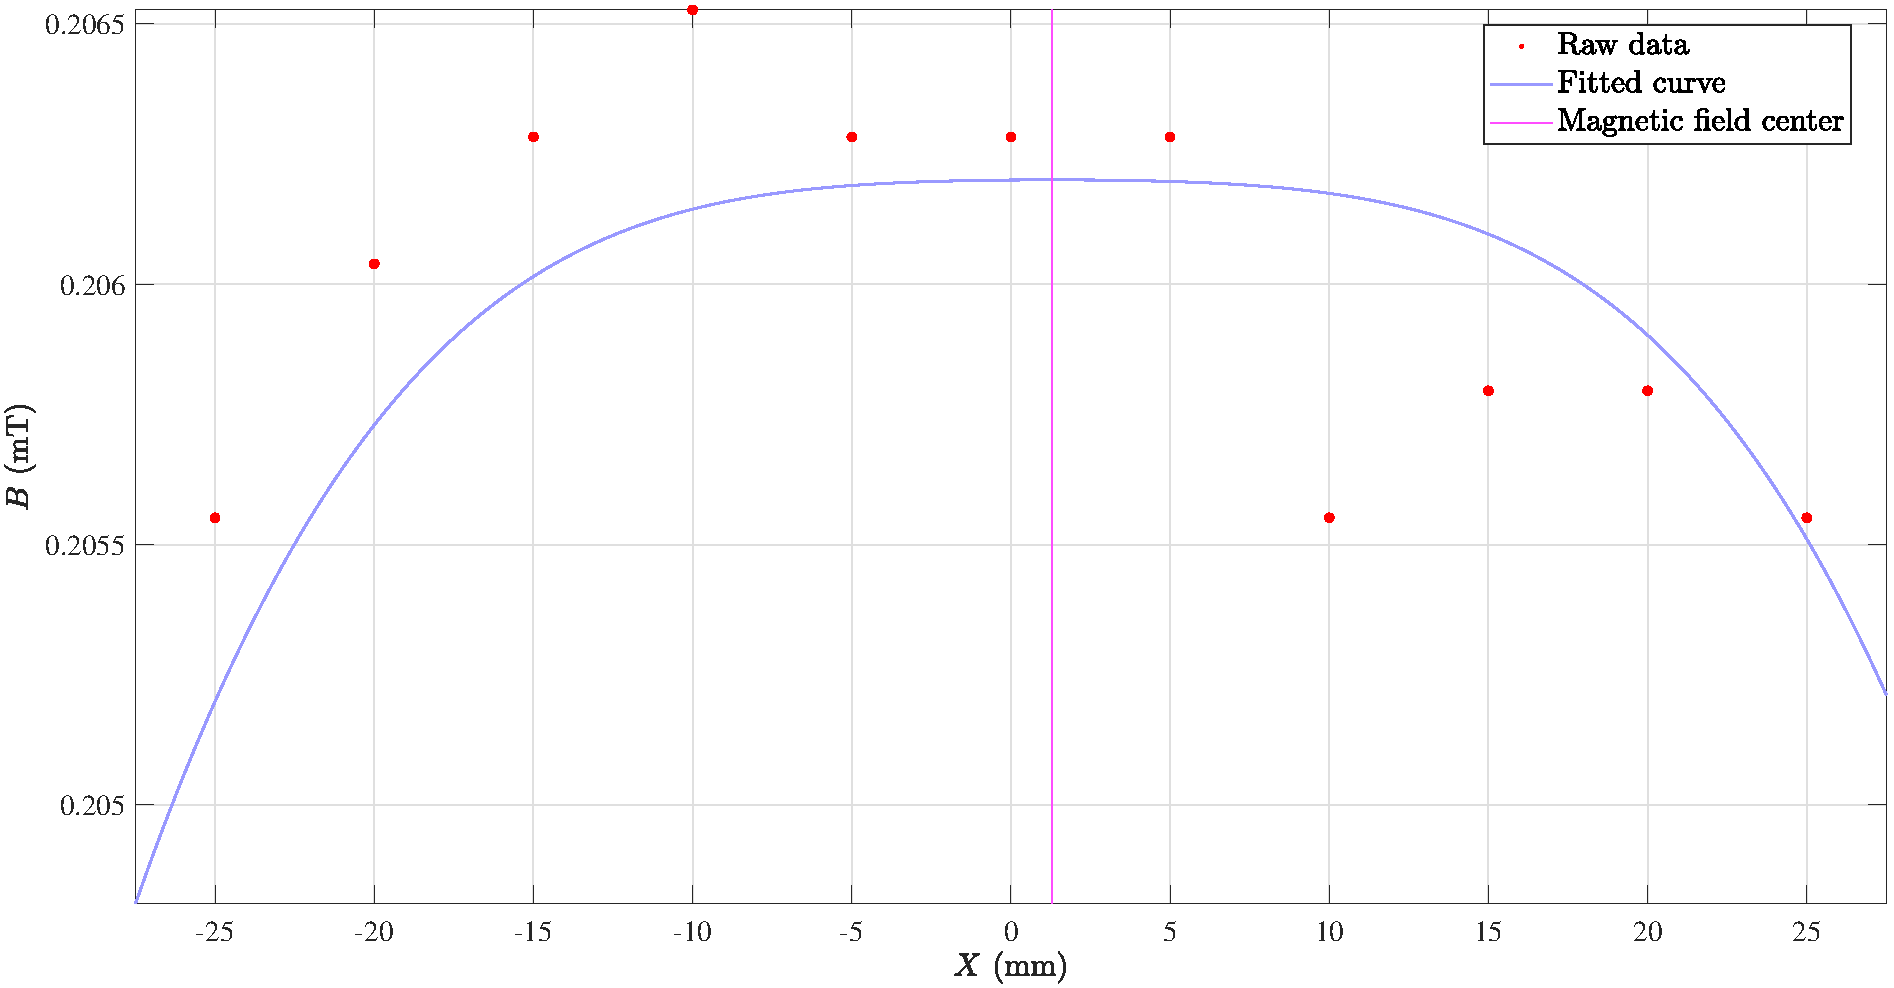
\includegraphics[scale=0.8]{7.png}
\end{figure}
我们从绘制的伏安特性曲线可以看出,16个测试点的线性程度很好,经最小二乘法拟合的线性相关系数为0.9925。拟合的电阻值为11.9kΩ


\begin{figure}[H]
    \centering
    \caption{数据表格}
    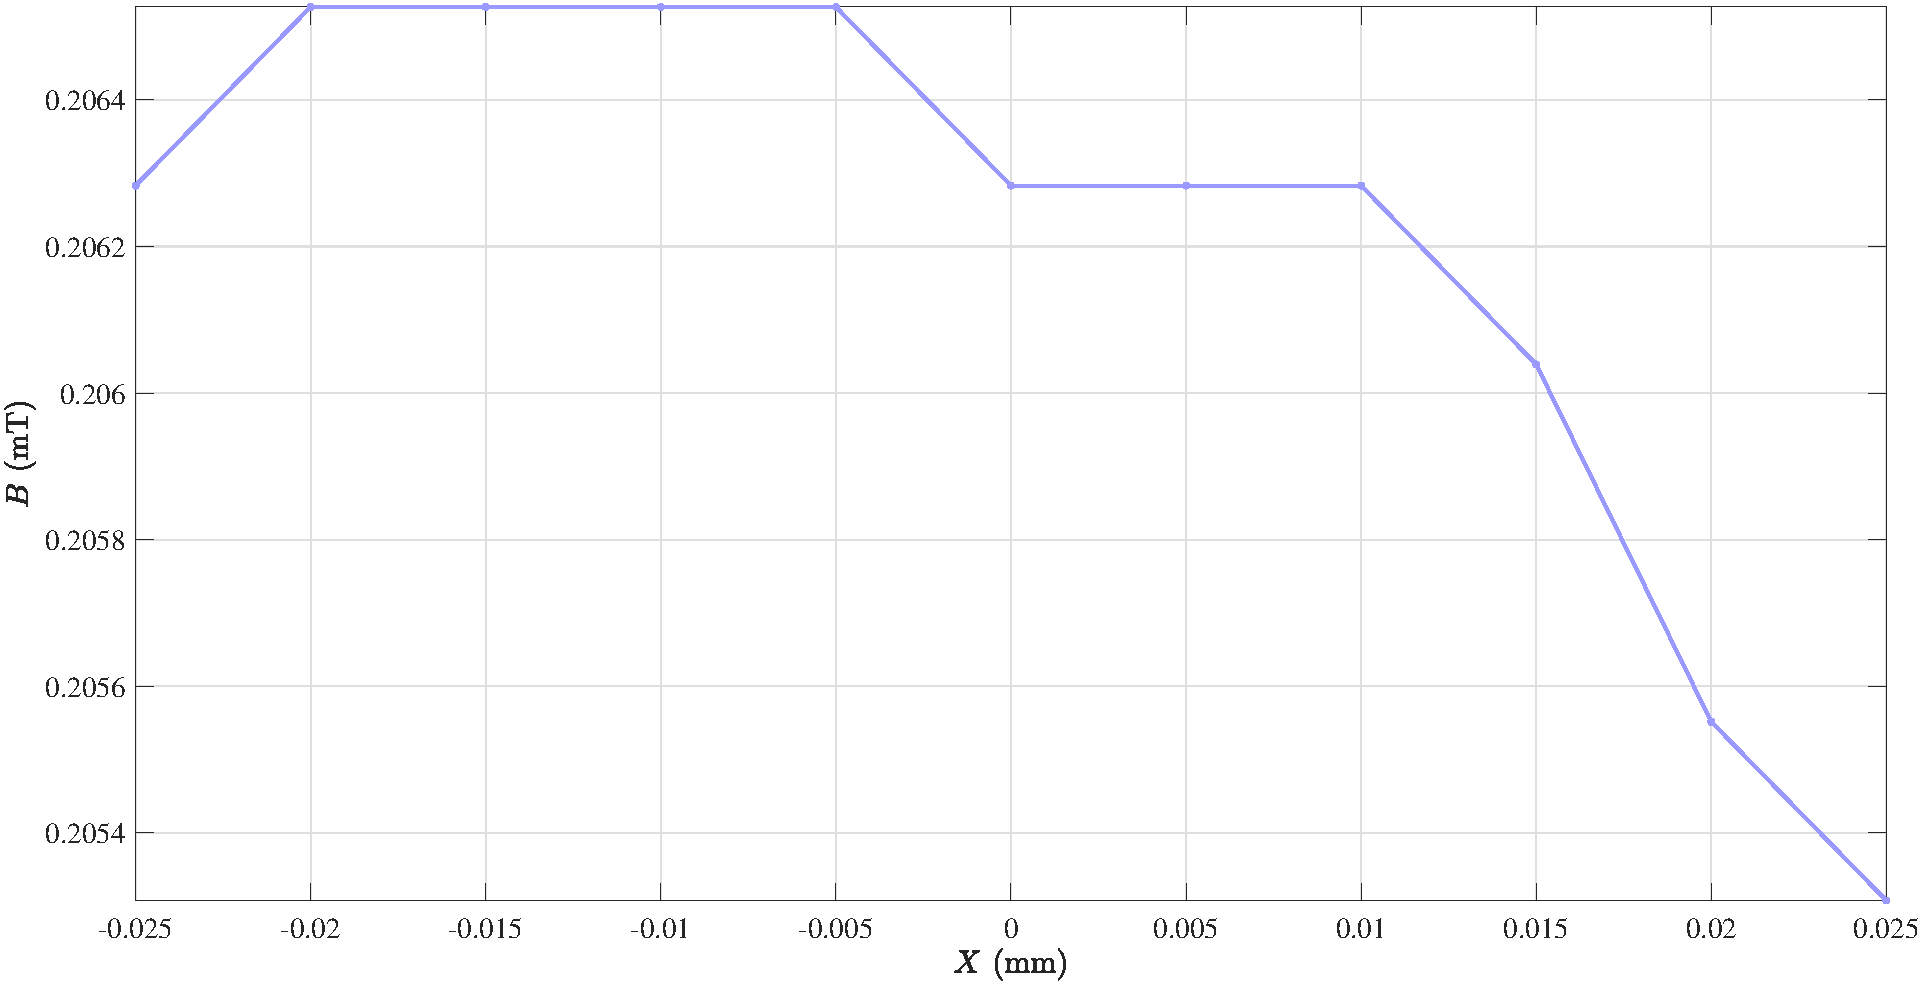
\includegraphics[scale=0.7]{8.png}
\end{figure}

\begin{figure}[H]
\centering
\caption{数据曲线}
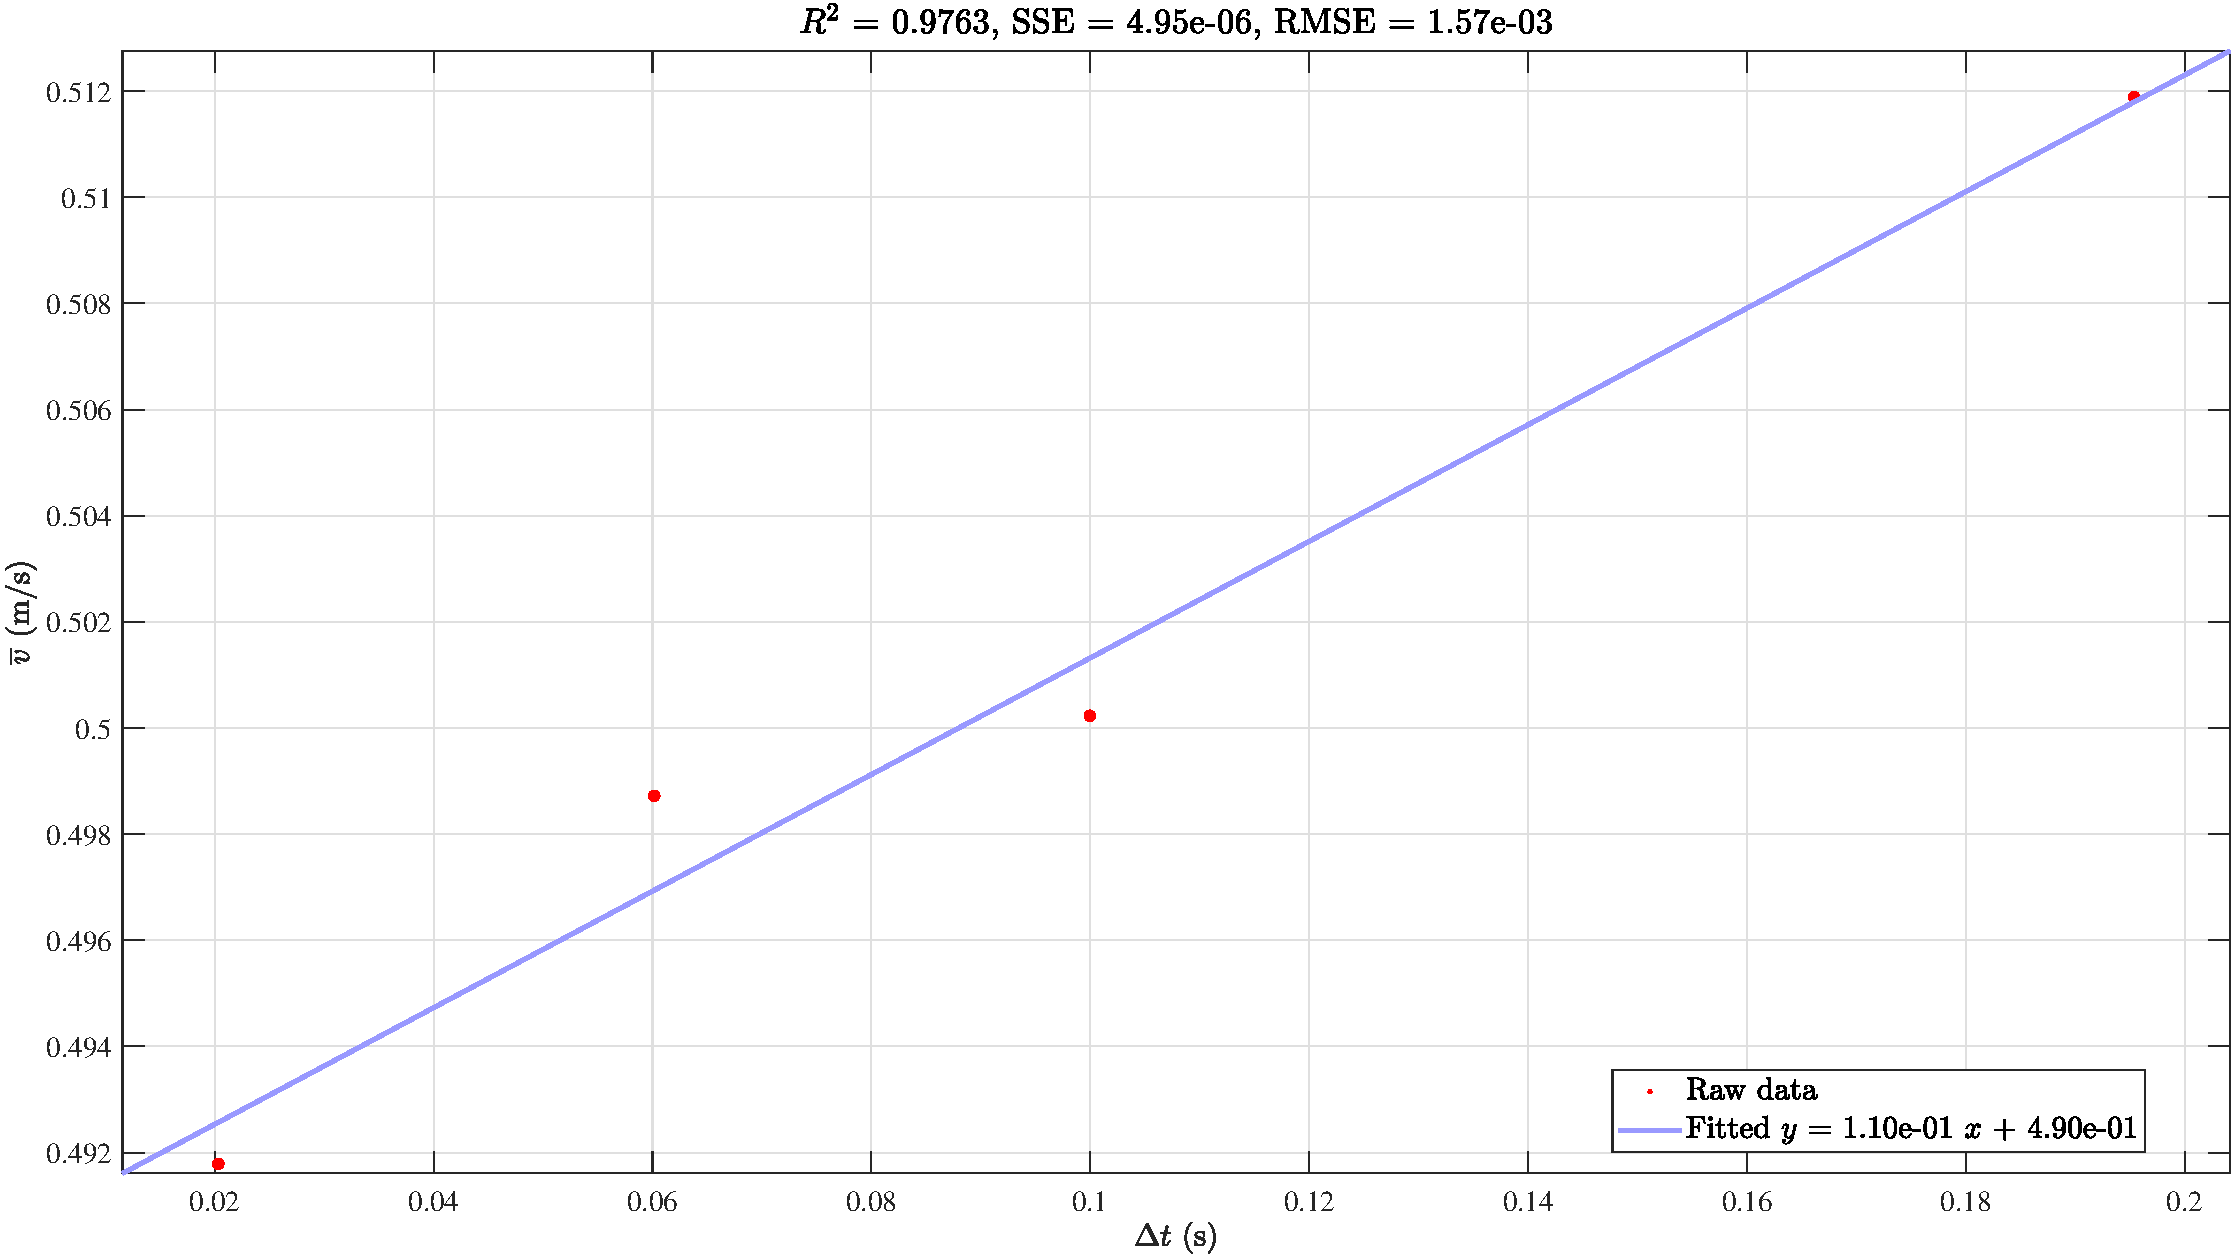
\includegraphics[scale=0.8]{9.png}
\end{figure}



我们从绘制的伏安特性曲线可以看出,18个测试点的线性程度极好,经最小二乘法拟合的线性相关系数几乎等于1,相当符合预期\par
拟合的电阻值为99Ω。\par

各种误差的产生原因可能如下:\par
1.电路板上的结构,包括连接导线和接触点之间,都可能会有一定的分布电阻,影响测量值大小\par
2.我们用虚拟仪器测量的电压和电流,在测量中充当电压表和电流表的结构也会对电路产生微小影响。


\begin{figure}[H]
    \centering
    \caption{数据表格}
    \includegraphics[scale=0.7]{11.png}
\end{figure}

\begin{figure}[H]
\centering
\caption{数据曲线}
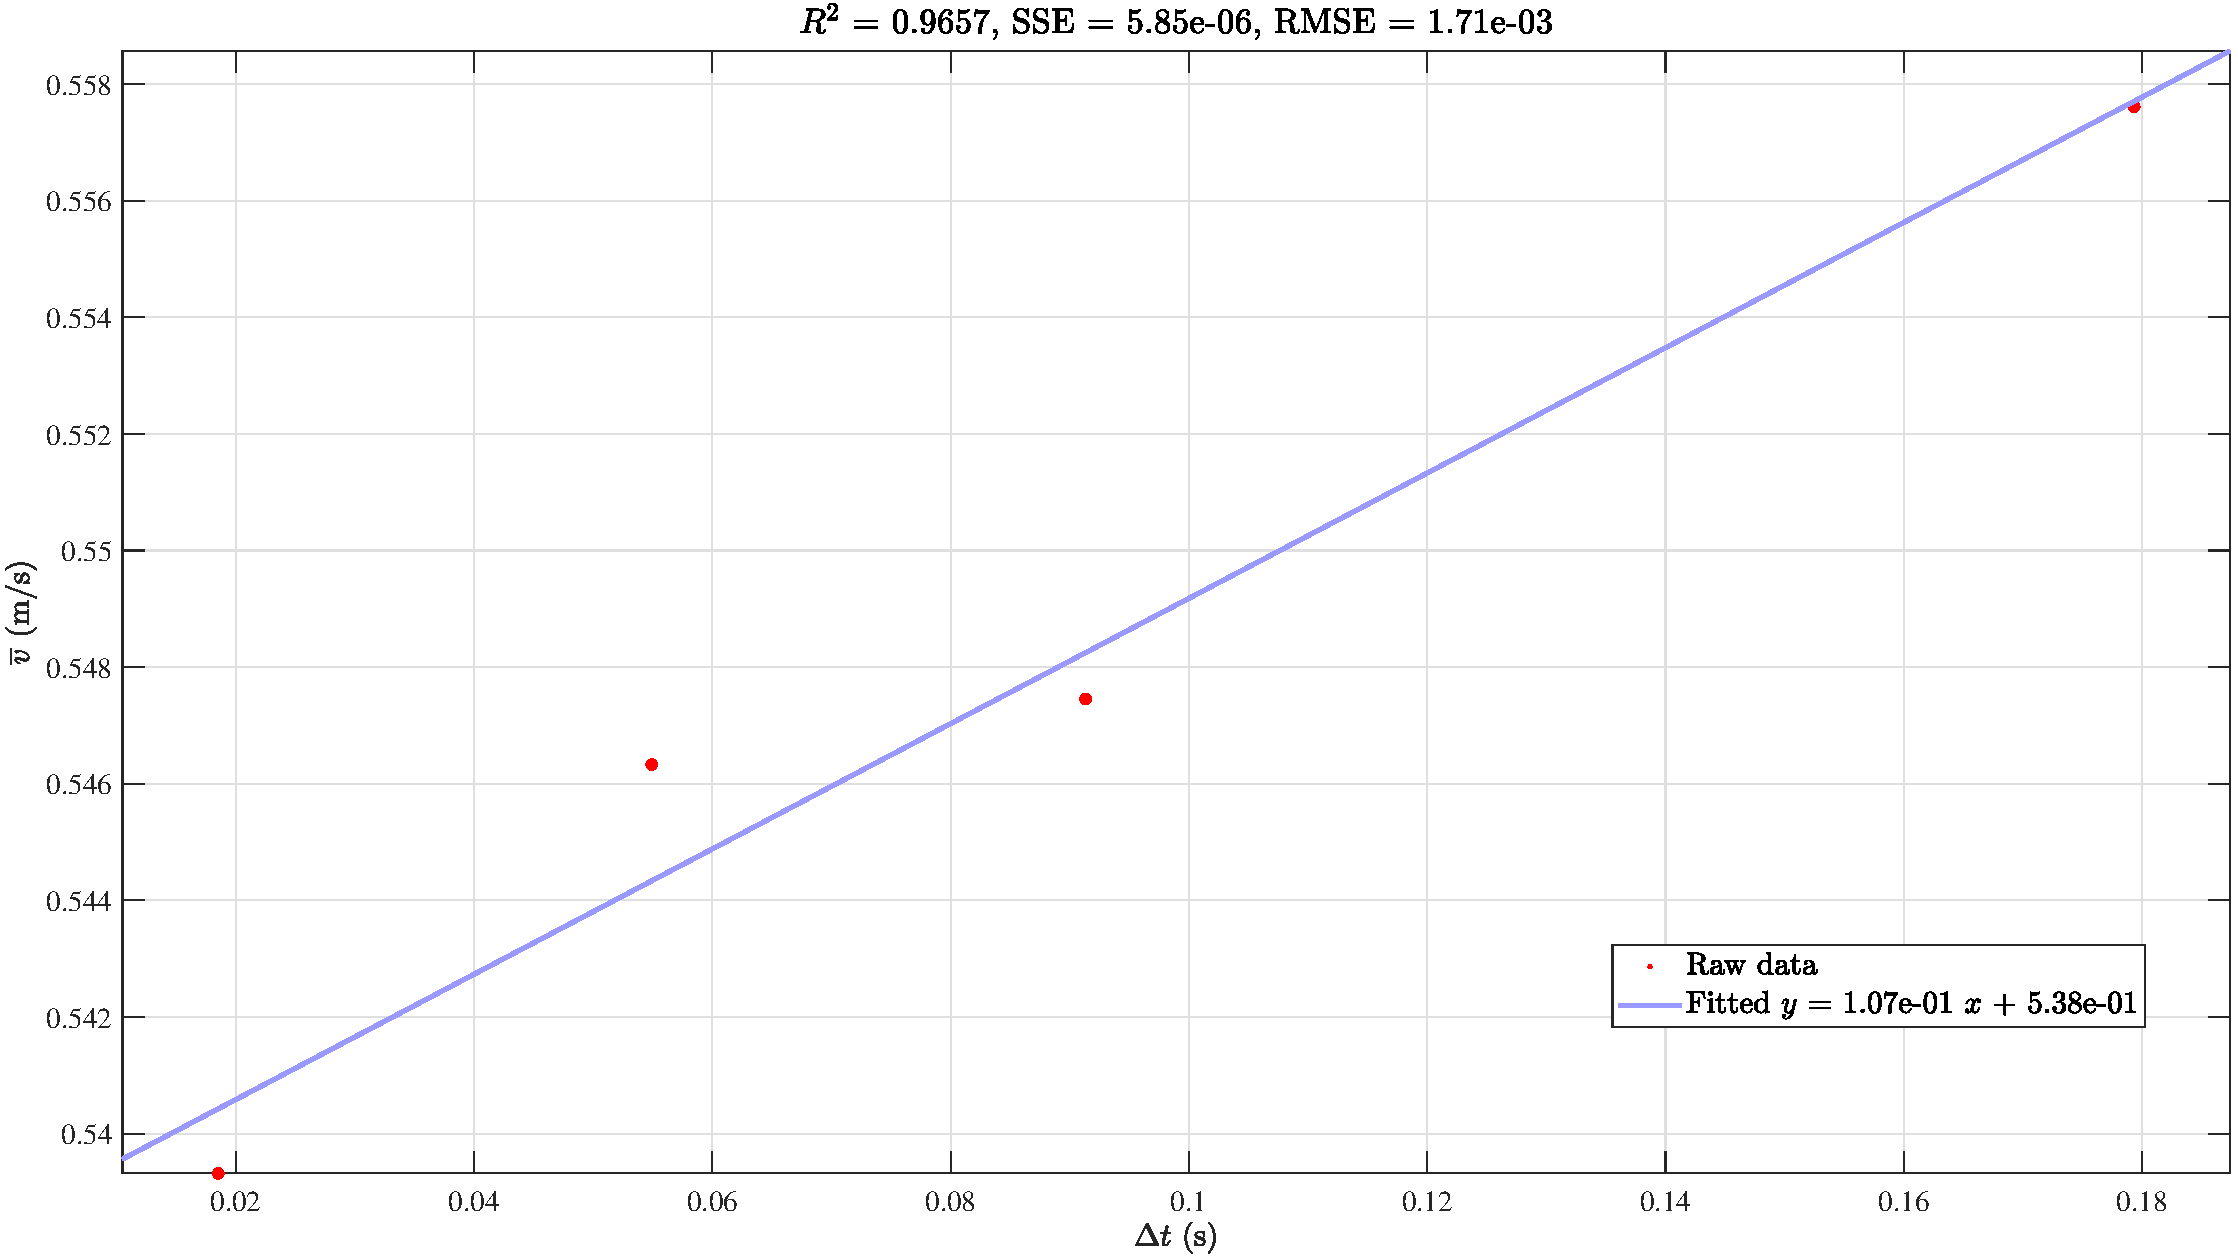
\includegraphics[scale=0.8]{10.png}
\end{figure}


可以看出二极管正向导通时,刚开始几乎不导通,当电压到达约0.5V左右,曲线显著攀升

\section{思考题}
    \subsubsection*{$\qquad1.$虚拟仪器系统与传统仪器有什么区别?请简要说明}
    硬件:虚拟仪器系统是基于计算机软件实现的,而传统仪器是基于硬件实现的。虚拟仪器系统不需要实体仪器,只需要一个计算机和相应的软件就可以实现测量和控制。

    软件:虚拟仪器系统的软件通常具有友好的用户界面和较高的自动化程度,可以帮助用户快速完成测量和分析。传统仪器则需要较长的学习和熟练的操作技能。

    灵活性:虚拟仪器系统具有较高的灵活性,可以根据用户需求定制功能。传统仪器的功能通常固定,不易修改。

    成本:虚拟仪器系统相比传统仪器的成本较低,可以降低实验室的开支,而且不需要耗费大量的时间和人力维护设备。

    可扩展性:虚拟仪器系统可以通过软件的更新和升级不断扩展和增强功能,而传统仪器则需要更换新的设备。
    \subsubsection*{$\qquad2.$本实验内容3中的电压输出和采集哪个先执行}
    物理通道程序运行前就搭建完毕,从本质上讲,开始运行后两个程序是并行的。两者的先后顺序仅由编译器来决定。因此,在通常情况下,两者开始执行的时间相差并不明显。
    我们可以将搭建好的虚拟仪器与传统仪器做类比,电压输出程序对应传统的电源,
    电压采集程序对应传统的电压表。因此,从实际应用上考虑,采用电压输出先执行,
    电压采集后执行,以避免开启电路时的缓冲对于测量结果的干扰。

\end{document}
